\documentclass[a4paper]{article}

\usepackage[margin=1in]{geometry}
\usepackage{amsfonts}
\usepackage{amsmath}
\usepackage{amssymb}
\usepackage{bm}
\usepackage[justification=centering]{caption}
\usepackage{float}
\usepackage{graphicx}
\usepackage{hyperref}
\usepackage[outputdir=out]{minted}
\usepackage{subcaption}
\usepackage{mdframed}

\def\sectionautorefname{Section}
\def\subsectionautorefname{Section}
\def\subsubsectionautorefname{Section}
\def\figureautorefname{Figure}
\def\tableautorefname{Table}
\def\equationautorefname{Equation}


\begin{document}

    \title{Bayesian Logistic Classification}
    \author{3F8: Inference Coursework \\ Theo Brown \\ Selwyn College, University of Cambridge}
    \date{\today}
    \maketitle

    \begin{abstract}
        Abstract goes here
    \end{abstract}

    \tableofcontents

    \section{Introduction}\label{sec:introduction}
  Classification is the task of grouping data points according to their shared features, and assigning each group a label.
  For a human with a small dataset, this is a trivial task, but it is much more difficult and slow with very large or complex data sets.
  Consequently, the development of good machine classifiers is an important area in statistical learning.
  Trained classifiers can be used as predictive tools to identify the most probable class that a new input will belong to, which could, for example, be useful in a medical setting, such as identifying the most at-risk patients.

    \section{Model definition}\label{sec:model-definition}
    \subsection{Logistic classification}
    The logistic classifier is a binary classifier that takes N D-dimensional inputs $\{\bm{x}_n\}$ and outputs class labels $\{y_n\}$, $y_i = \{0, 1\}$, where the class labels are modelled as being independent and identically generated from a Bernoulli distribution:
    \begin{align}
        p(y_n = 1 | \tilde{\bm{x}}_n) &= \sigma (\bm{w}^T\tilde{\bm{x}}_n) \nonumber \\
        p(y_n = 0 | \tilde{\bm{x}}_n) &= 1 - \sigma (\bm{w}^T\tilde{\bm{x}}_n) = \sigma (-\bm{w}^T\tilde{\bm{x}}_n)
        \label{eq:logistic-classifier}
    \end{align}
    with $\tilde{\bm{x}}_n = \left[1, \bm{x}_n^T \right]^T$, $\bm{w}$ as a vector of D+1 model weights, and $\sigma(x) = \frac{1}{1 + e^{-x}}$ (the logistic function).

    \subsection{Bayesian logistic classification}
    A posterior distribution of the model weights is required to perform fully Bayesian classification:
    \begin{align}
        p(\bm{w} | \bm{X}, \bm{y}) = \frac{p(\bm{X} | \bm{w}, \bm{y}) p(\bm w)}{p(\bm{X} | \bm{y})}
        \label{eq:posterior}
    \end{align}
    From the definition of the logistic classifier, the log-likelihood of \textbf{w} is:
    \begin{align}
        \mathcal{L}(\bm{w}) = \log p(y|\tilde{\bm{X}}, \bm{w})
        &= \log \prod_{n=1}^{N} \sigma( \bm{w}^T \tilde{\bm{x}}_n)^{y_n}
        \sigma (-\bm{w}^T \tilde{\bm{x}}_n)^{1-y_n} \nonumber \\
        &= \sum_{n=1}^{N} y_n \log\sigma( \bm{w}^T \tilde{\bm{x}}_n) + (1-y_n) \log\sigma(-w^T \tilde{\bm{x}}_n)
        \label{eq:log-likelihood}
    \end{align}
    The prior distribution of the model weights is chosen to be Gaussian, $p(\bm{w}) = \mathcal{N}(\bm{w}; \bm{m}_0, \bm{S}_0)$.
    This gives the log-prior as:
    \begin{align}
        \mathcal{P}(\bm{w}) = \log p(\bm{w}) = -\frac{1}{2}(\bm{w} - \bm{m}_0)^T \bm{S}_0^{-1} (\bm{w} - \bm{m}_0) + \text{const}
        \label{eq:log-prior}
    \end{align}
    The log-posterior is:
    \begin{align}
        \log p(\bm{w} | \bm{X}, \bm{y}) = \mathcal{L}(\bm{w}) + \mathcal{P}(\bm{w}) + \text{const}
        \label{eq:log-posterior}
    \end{align}

    Calculating the model evidence $p(\bm{X} | \bm{y})$ exactly requires integrating the product of the likelihood and the prior, which is intractable.
    We present two methods to circumvent this problem: MAP estimation and the Laplace approximation. The performance of these methods is discussed in \autoref{sec:performance}.

    \subsubsection{`Semi-Bayesian' classification: MAP estimation}
    One method of performing Bayes-driven logistic classification is to use the MAP estimate of the model weights, $\bm{w_\text{MAP}}$, which can be found by applying gradient ascent to the log-posterior.
    This method does not require the model evidence, but discards a lot of the information contained in the posterior and does not give a distribution of the model weights.
    As such, it is not `true' Bayesian classification.
    The gradient of the log-posterior is calculated as follows:
    \begin{align}
        \frac{\partial}{\partial \bm{w}} \log p(\bm{w} | \tilde{\bm{X}}, \bm{y}) &= \frac{\partial}{\partial \bm{w}} \mathcal{L}(\bm{w}) + \frac{\partial}{\partial \bm{w}} \mathcal{P}(\bm{w}) \nonumber \\
        &= \sum_{n=1}^{N} \left(y_n - \sigma(\bm{w}^T \tilde{\bm{x}}_n) \right)  \tilde{\bm{x}}_n  + \bm{S}_0^{-1}(\bm{w} - \bm{m}_0) \nonumber \\
        &= \tilde{\bm{X}} (\textbf{y} - \sigma(\tilde{\bm{X}}^T \bm{w})) +  \bm{S}_0^{-1}(\bm{w} - \bm{m}_0)
        \label{eq:log-posterior-gradient}
    \end{align}
    where $\tilde{\bm{X}} = [\tilde{\bm{x}}_1 \dots \tilde{\bm{x}}_N]$.
    A standard gradient-based solver can be used with \autoref{eq:log-posterior-gradient} to find a value for $\bm{w}_\text{MAP}$, which can be used as a setting for the weights in \autoref{eq:logistic-classifier} to classify data points.

    \subsubsection{`True' Bayesian classification: the Laplace approximation}
    The Laplace approximation allows us to perform `true' Bayesian classification.
    In this method, approximations to the posterior distribution and the model evidence can be found by finding a Gaussian distribution $q(\bm{w})$ that closely models the posterior $p(\bm{w} | \tilde{\bm{X}}, \bm{y})$ around a local maximum.
    The normalising constant of a Gaussian is well defined, so the calculation of the approximate model evidence is simple.
    For brevity, rewrite \autoref{eq:posterior} as:
    \begin{align}
        p(\bm{w} | \bm{X}, \bm{y}) = \frac{f(\bm{w})}{K} \approx q(\bm{w}) \nonumber
    \end{align}
    where $f(\bm{w}) = p(\bm{X} | \bm{w}, \bm{y}) p(\bm{w})$ and $K = p(\bm{X} | \bm{y}) = \int f(\bm{w}) d\bm{w}$.

    \vspace{\baselineskip}
    \noindent\textbf{Approximate log-posterior} \\
    \noindent To find $q(\bm{w})$, we start with the truncated Taylor expansion of $\log f(\bm{w})$ around a local maximum $\bm{w}_0$:
    \begin{align}
        \nonumber
        \log f(\bm{w}) &\approx \log f(\bm{w}_0) + \nabla \log f(\bm{w}) \big|_{\bm{w} = \bm{w}_0} (\bm{w} - \bm{w}_0)
        + \frac{1}{2} (\bm{w} - \bm{w}_0)^T \nabla^2 \log f(\bm{w}) \big|_{\bm{w} = \bm{w}_0} (\bm{w} - \bm{w}_0)
    \end{align}
    At a maximum of $f(\bm{w})$, $\nabla \log f(\bm{w}) = 0$ as the logarithm is a monotonic function.
    Hence, close to $\bm{w}_0$:
    \begin{align}
        \log f(\bm{w}) \approx \log f(\bm{w}_0) + \frac{1}{2} (\bm{w} - \bm{w}_0)^T \nabla^2 \log f(\bm{w}) \big|_{\bm{w} = \bm{w}_0} (\bm{w} - \bm{w}_0) \nonumber \\
        f(\bm{w}) \approx f(\bm{w}_0) \exp \left(\frac{1}{2} (\bm{w} - \bm{w}_0)^T \nabla^2 \log f(\bm{w}) \big|_{\bm{w} = \bm{w}_0} (\bm{w} - \bm{w}_0) \right) \nonumber
    \end{align}
   This is of the form of an un-normalised Gaussian centred on the maximum at $\bm{w}_0$.
    Set $\bm{w}_0 = \bm{w}_\text{MAP}$, and let $\bm{S}_N^{-1} = -\nabla^2 \log f(\bm{w})\big|_{\bm{w} = \bm{w}_\text{MAP}}$,
    then normalise to obtain the approximate posterior distribution:
    \begin{align}
        p(\bm{w} | \tilde{\bm{X}}, \bm{y}) &\approx \frac{1}{(2\pi)^\frac{N}{2} \det\bm{S}_N^{-\frac{1}{2}}} \exp \left(\frac{1}{2} (\bm{w} - \ \bm{w}_\text{MAP})^T \bm{S}_N^{-1} (\bm{w} -  \bm{w}_\text{MAP}) \right) \nonumber \\
        &= \mathcal{N}(\bm{w};  \bm{w}_\text{MAP}, \bm{S}_N)
        \label{eq:approximate-posterior}
    \end{align}
    where N is the number of data points $\bm{x}_n$.
    For \autoref{eq:approximate-posterior} to hold, $\bm{S}_N^{-1}$ must be positive definite, which is equivalent to saying $\bm{w}_\text{MAP}$ must be a maximum (which is true by definition).

    \vspace{\baselineskip}
    \noindent\textbf{Approximate log-evidence} \\
    Now we can obtain an approximate value of the normalising constant K, by substituting \autoref{eq:approximate-posterior} into the definition of K:
    \begin{align}
        K = \int f(\bm{w}) d\bm{w} &\approx f(\bm{w}_0) \int \exp \left(\frac{1}{2} (\bm{w} - \bm{w}_0)^T \bm{S}_N^{-1} (\bm{w} - \bm{w}_0) \right) d\bm{w} \nonumber \\
        &= \sqrt{\frac{(2\pi)^N}{\det \bm{S}_N}} f(\bm{w}_0) \nonumber
    \end{align}
    Taking logs and substituting in the definitions of $\bm{w}_0$, $K$, and $f(\bm{w})$ gives the approximate log-evidence:
    \begin{align}
        \log p(\bm{X} | \bm{y}) &\approx  \frac{N}{2}\log 2\pi - \frac{1}{2}\log \det \bm{S}_N + \mathcal{L}(\bm{w}_\text{MAP}) + \mathcal{P}(\bm{w}_\text{MAP})
        \label{eq:approximate-log-evidence}
    \end{align}

    \vspace{\baselineskip}
    \noindent\textbf{Covariance matrix} \\
    Differentiating \autoref{eq:log-posterior-gradient}, the covariance matrix of $q(\bm{w})$ can be found:
    \begin{align}
        \bm{S}_N^{-1} &= -\nabla^2 \log p(\bm{w} | \bm{X}, \bm{y}) \big|_{\bm{w} = \bm{w}_{\text{MAP}}} \nonumber \\
        &= -\nabla^2 \mathcal{P}(\bm{w}) \big|_{\bm{w} = \bm{w}_{\text{MAP}}} -\nabla^2 \mathcal{L}(\bm{w})\big|_{\bm{w} = \bm{w}_{\text{MAP}}} \nonumber \\
        &= \bm{S}_0^{-1}
        + \sum_{n=1}^N \sigma(\bm{w}^T \tilde{\bm{x}}_n) \sigma(-\bm{w}^T \tilde{\bm{x}}_n)\tilde{\bm{x}}_n\tilde{\bm{x}}_n^T
        \label{eq:covariance-matrix}
    \end{align}

    \vspace{\baselineskip}
    \noindent\textbf{Predictive distribution} \\
    The predictive distribution can also be approximated using the Laplace approximation for the posterior:
    \begin{align}
        p(y^* = 1 | \bm{x}^*, \bm{y}, \bm{X}) &= \int p(y^* = 1 | \bm{x}^*, \bm{w}) p(\bm{w} | \bm{y}, \bm{X}) d\bm{w} \nonumber \\
        & \approx \int \sigma(\bm{w}^T\bm{x}^*) q(\bm{w}) d\bm{w} \nonumber
    \end{align}
    Using the sifting property of the delta function:
    \begin{align}
        \sigma(\bm{w}^T \bm{x}) = \int \delta(a - \bm{w}^T \bm{x}) \sigma(a) da \nonumber
    \end{align}
    Hence:
     \begin{align}
        p(y^* = 1 | \bm{x}^*, \bm{y}, \bm{X}) &\approx \int \int \delta(a - \bm{w}^T \bm{x}^*) \sigma(a) q(\bm{w}) d\bm{w} da \nonumber \\
         &= \int \sigma(a) \int \delta(a - {\bm{x}^*}^T \bm{w}) q(\bm{w}) d\bm{w} da \nonumber
    \end{align}
    The inner integral applies a linear constraint to $q(\bm{w})$, as the argument of the delta function is 0 unless $a = {\bm{x}^*}^T \bm{w}$.
    Hence, the approximate predictive distribution is:
    \begin{align}
        \label{eq:intermediate-approx-predictive}
         p(y^* = 1 | \bm{x}^*, \bm{y}, \bm{X}) &\approx \int \sigma(a) \mathcal{N}(a; {\bm{x}^*}^T \bm{w}_\text{MAP}, {\bm{x}^*}^T \bm{S}_N \bm{x^*}) da \nonumber \\
        &= \int \sigma(a) \mathcal{N}(a; \mu_p, \sigma_p^2) da
     \end{align}
    \begin{align*}
        \mu_p &= {\bm{x}^*}^T \bm{w}_\text{MAP}\\
        \sigma_p^2 &= {\bm{x}^*}^T \bm{S}_N \bm{x^*}
    \end{align*}
    This integral cannot be expressed analytically, so another approximation is required.
    The logistic function can be approximated well by a probit function scaled such that the gradient of the two functions at the origin are equal.
    It can be shown that this gives:
    \begin{align}
        \label{eq:probit-approximation}
        \sigma(x) \approx \Phi^{-1}\left(\sqrt{\frac{\pi}{8}} x\right) = \Phi^{-1}(\lambda x)
    \end{align}
    Substituting into \autoref{eq:intermediate-approx-predictive} and evaluating using properties of the probit function gives:
    \begin{align*}
         p(y^* = 1 | \bm{x}^*, \bm{y}, \bm{X}) &\approx \int \Phi^{-1}(\lambda x) \mathcal{N}(a; \mu_p, \sigma_p) da \nonumber \\
        &= \Phi^{-1}\left(\frac{\mu_p}{\sqrt{\lambda^{-2} + \sigma_p^2}}\right)
     \end{align*}
    Using \autoref{eq:probit-approximation}, this can be converted back into a logistic function:
    \begin{align}
        \label{eq:approximate-predictive}
         p(y^* = 1 | \bm{x}^*, \bm{y}, \bm{X}) &\approx \sigma\left(\frac{\mu_p}{\sqrt{1 + \sigma_p^2\lambda^2}}\right)
    \end{align}

    \begin{mdframed}
    \noindent\textbf{Summary of Laplace Approximation} \\
    \begin{itemize}
        \item Posterior distribution of $\bm{w}$:
        \begin{align*}
            p(\bm{w} | \bm{X}, \bm{y}) \approx \mathcal{N}(\bm{w}; \bm{w}_\text{MAP}, \bm{S}_N) \tag{\ref{eq:approximate-posterior} restated}
        \end{align*}
        \begin{align*}
            \bm{S}_N = \bm{S}_0^{-1} + \sum_{n=1}^N \sigma(\bm{w}^T \tilde{\bm{x}}_n) \sigma(-\bm{w}^T \tilde{\bm{x}}_n) \tilde{\bm{x}}_n\tilde{\bm{x}}_n^T \tag{\ref{eq:covariance-matrix} restated}
        \end{align*}
        \item Model evidence:
        \begin{align}
            \log p(\bm{X} | \bm{y}) &\approx  \frac{N}{2}\log 2\pi - \frac{1}{2}\log \det \bm{S}_N + \mathcal{L}(\bm{w}_\text{MAP}) + \mathcal{P}(\bm{w}_\text{MAP})
                \tag{\ref{eq:approximate-log-evidence} restated}
        \end{align}
        \item Predictive distribution for new points $\bm{x}_*$:
        \begin{align*}
            p(y_* = 1 | \bm{x}_*, \bm{y}, \bm{X}) &\approx \sigma\left(\frac{\mu_p}{\sqrt{1 + \sigma_p^2\lambda^2}}\right) \tag{\ref{eq:approximate-predictive} restated} \\
            p(y_* = 0 | \bm{x}_*, \bm{y}, \bm{X}) &= 1 - p(y_* = 1 | \bm{x}_*, \bm{y}, \bm{X}) \nonumber
        \end{align*}
            \begin{align*}
        \mu_p &= {\tilde{\bm{x}}_*}^T \bm{w}_\text{MAP} \\
        \sigma_p^2 &= {\tilde{\bm{x}}_*}^T \bm{S}_N \tilde{\bm{x}}_* \\
        \lambda^2 &= \frac{\pi}{8}
    \end{align*}
    \end{itemize}
    \end{mdframed}

    \section{Implementation in Python}
    Firstly, the data is loaded and split into training and test sets:
    \begin{minted}{python}
    import numpy as np
    from sklearn.model_selection import train_test_split
    from sklearn.utils import shuffle

    X_data, y_data = shuffle(np.loadtxt('data/X.txt'),
                             np.loadtxt('data/y.txt'))

    X_train, X_test, y_train, y_test = train_test_split(X_data, y_data, train_size=800)
    \end{minted}
    Some utility functions are defined, include the function that expands the inputs through radial basis functions (RBFs) to allow for non-linear decision boundaries:
    \begin{minted}{python}
    def log(x, epsilon=1e-5):
        """Log function that avoids divide by zero errors"""
        return np.log(x + epsilon)

    def prepend_ones(M):
        return np.column_stack((np.ones(M.shape[0]), M))

    def expand_inputs(width, data, centers=X_train):
        """Expand data through a set of RBFs with given centres and widths"""
        l = width
        Z = centers
        X = data
        X2 = np.sum(X**2, 1)
        Z2 = np.sum(Z**2, 1)
        ones_Z = np.ones(Z.shape[ 0 ])
        ones_X = np.ones(X.shape[ 0 ])
        r2 = np.outer(X2, ones_Z) - 2 * np.dot(X, Z.T) + np.outer(ones_X, Z2)
        return prepend_ones(np.exp(-0.5 / l**2 * r2))
    \end{minted}
    Next, the central equations of the model are defined. In this implementation, we consider a uniform prior on the weights with mean $0$ and covariance $\bm{I}\sigma_0^2$:
    \begin{align}
        p(\bm{w}) &= \mathcal{N}(\bm{w}; 0, \bm{I}\sigma_0^2) \label{eq:prior} \\
        \mathcal{P}(\bm{w}) &\propto -\frac{1}{2\sigma_0^2} \bm{w}^T\bm{w} \nonumber
    \end{align}
    \begin{minted}{python}
    def logistic(x):
        return 1 / (1 + np.exp(-x))

    def log_prior(w, variance):
        return -1 / (2 * variance) * (w.T @ w)

    def log_likelihood(w, X, y):
        sigma = logistic(X @ w)
        return np.sum(y * log(sigma)
                      + (1 - y) * log(1 - sigma))

    def log_likelihood_gradient(w, X, y):
        return (y - logistic(X @ w)) @ X

    def log_posterior(w, X, y, prior_variance):
        return log_likelihood(w, X, y) + log_prior(w, prior_variance)

    def posterior_gradient(w, X, y, prior_variance):
        return (y - logistic(X @ w)) @ X - w / prior_variance
    \end{minted}
    We use gradient descent to find the MAP and maximum likelihood estimates of the weights:
    \begin{minted}{python}
    from scipy.optimize import fmin_l_bfgs_b as minimise

    def find_w_map(X, y, prior_variance, w0):
        w_map, *d = minimise(lambda w, X, y, prior_variance:
                                -log_posterior(w, X, y, prior_variance),
                             w0,
                             lambda w, X, y, prior_variance:
                                -posterior_gradient(w, X, y, prior_variance),
                             args=[X, y, prior_variance])
        return w_map

    def find_w_ml(X, y, w0):
        w_ml, *d = minimise(lambda w, X, y: -log_likelihood(w, X, y),
                            w0,
                            lambda w, X, y: -log_likelihood_gradient(w, X, y),
                            args=[X, y])
        return w_ml


    \end{minted}
    Note that \verb`scipy.optimize.fmin_l_bfgs_b` is a minimisation function, so to maximise $f(x)$ we have to work with $-f(x)$ and $-\nabla f(x)$.

    Once $\bm{w}_{\text{MAP}}$ is found, the Laplace approximation for the model evidence and the predictive distribution can be found. First we find the Hessian matrix $S_N$ using \autoref{eq:covariance-matrix}:
    \begin{minted}{python}
    def calculate_hessian(weights, rbf_width, prior_variance):
        # The Hessian will be MxM, where M is the number of features (= D+1)
        M = weights.shape[0]

        X_tilde = expand_inputs(rbf_width, X_train)

        # Contribution from prior
        h = np.identity(M) / prior_variance

        # Contribution from data
        for x in X_tilde:
            sigma = logistic(weights @ x)
            h += sigma * (1 - sigma) * np.outer(x, x)

        return h
    \end{minted}
    Then the predictive function (\autoref{eq:approximate-predictive}) can be implemented:
    \begin{minted}{python}
    def laplace_prediction(inputs, weights, rbf_width, prior_variance):
        X_tilde = expand_inputs(rbf_width, X_train)
        sigma = logistic(X_tilde @ weights)
        S_N = np.linalg.inv(calculate_hessian(weights, rbf_width, prior_variance))
        predictive_mean = inputs @ weights
        predictive_variance = np.array([x.T @ S_N @ x for x in inputs])
        return logistic(predictive_mean / np.sqrt(1 + predictive_variance*np.pi/8))
    \end{minted}
    The approximate log-evidence is calculated using \autoref{eq:approximate-log-evidence}. The log-determinant is calculated using \verb`np.linalg.slogdet`, which helps avoid the numerical errors encountered when calculating the determinant directly:
    \begin{minted}{python}
    def log_evidence(w, X, y, rbf_width, prior_variance):
        h = calculate_hessian(w, rbf_width, prior_variance)
        sign, logdet = np.linalg.slogdet(h)
        if np.exp(logdet) == 0:
            # If the determinant is 0, the approximation does not work
            return -np.inf
        return ((y.size/2)*log(2*np.pi)
                - 0.5*logdet
                + log_likelihood(w, X, y)
                + log_prior(w, prior_variance))
    \end{minted}

    \section{Performance of the Laplace Approximation}\label{sec:performance}
    \subsection{Comparison with MAP and ML estimates}
    \subsubsection{Predictive distributions}
    The predictive distributions calculated using the ML estimate, MAP estimate, and Laplace approximation are shown in \autoref{fig:predictive-distributions-width-0.1} and \autoref{fig:predictive-distributions-width-1}.
    The predictive distribution based on the ML estimate is visibly inferior to those generated by the MAP estimate and Laplace approximation, and exhibits signs of overfitting (boundaries very tight around some data points in \autoref{fig:predictive-distribution-ml-width-0.1}, spurious classification regions far from data in \autoref{fig:predictive-distribution-ml-width-1}).
    The probability contours in the Laplace predictive distribution are slightly more spread out than the ones in the MAP distribution, defining less sharp boundaries between the classes and lower confidence far away from data points.
    This effect is more pronounced for larger RBF widths (\autoref{fig:predictive-distributions-width-1}): the distribution in \autoref{fig:predictive-distribution-laplace-width-1} extends slightly less far from the data compared to \autoref{fig:predictive-distribution-map-width-1}.
    It is likely that optimising the parameters of the Laplace approximation would improve this result further (see \autoref{sec:optimisation}).

    \begin{figure}[h]
        \begin{subfigure}{0.33\textwidth}
            \centering
            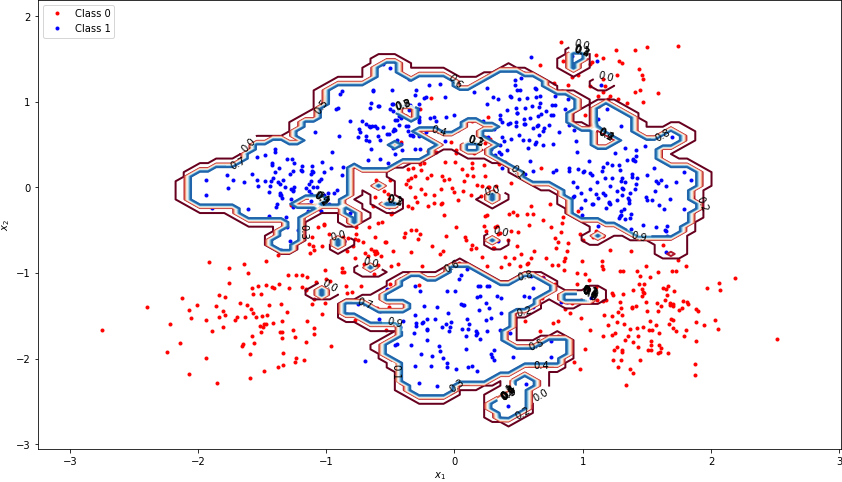
\includegraphics[width=\textwidth]{plots/bayesian_logistic_classification/predictive_distribution_ML_width_0.1}
            \caption{Maximum Likelihood estimate}
            \label{fig:predictive-distribution-ml-width-0.1}
        \end{subfigure}
        \begin{subfigure}{0.33\textwidth}
            \centering
            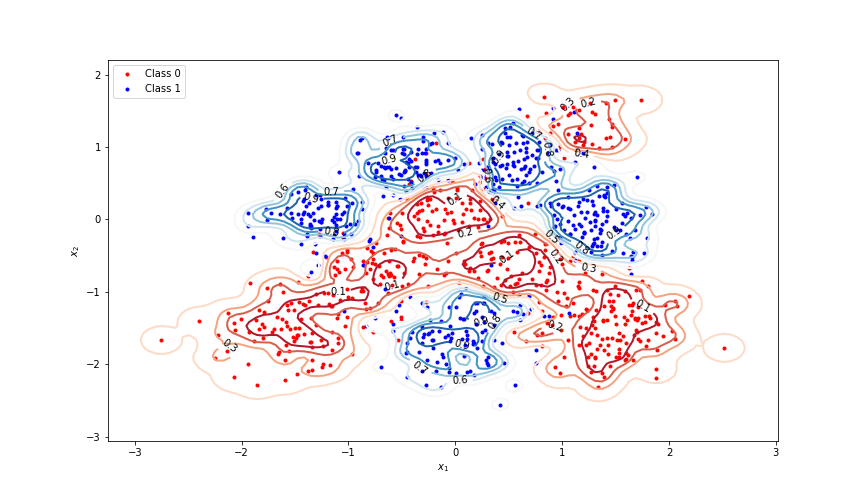
\includegraphics[width=\textwidth]{plots/bayesian_logistic_classification/predictive_distribution_MAP_width_0.1_prior_variance_1}
            \caption{MAP estimate ($\sigma_0^2=1$)}
            \label{fig:predictive-distribution-map-width-0.1}
        \end{subfigure}
        \begin{subfigure}{0.33\textwidth}
            \centering
            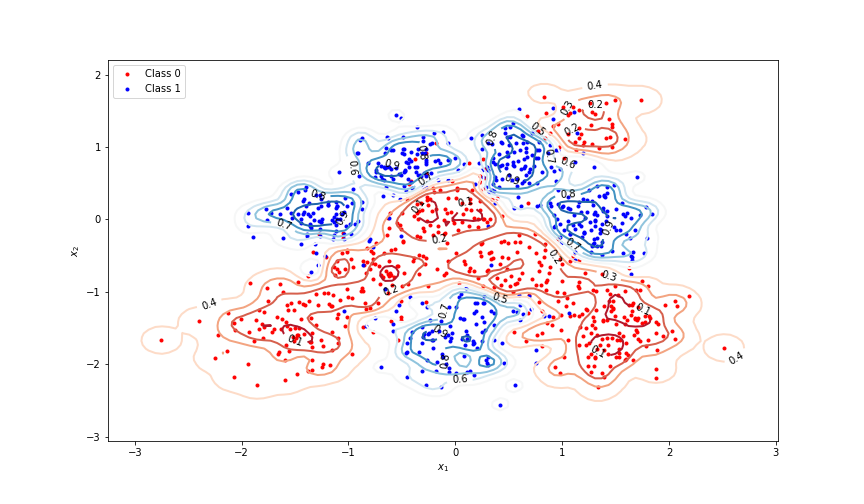
\includegraphics[width=\textwidth]{plots/bayesian_logistic_classification/predictive_distribution_laplace_width_0.1_prior_variance_1}
            \caption{Laplace approximation ($\sigma_0^2=1$)}
            \label{fig:predictive-distribution-laplace-width-0.1}
        \end{subfigure}
        \caption{Predictive distributions, RBF width = $0.1$}
        \label{fig:predictive-distributions-width-0.1}
    \end{figure}
\begin{figure}[h]
        \begin{subfigure}{0.33\textwidth}
            \centering
            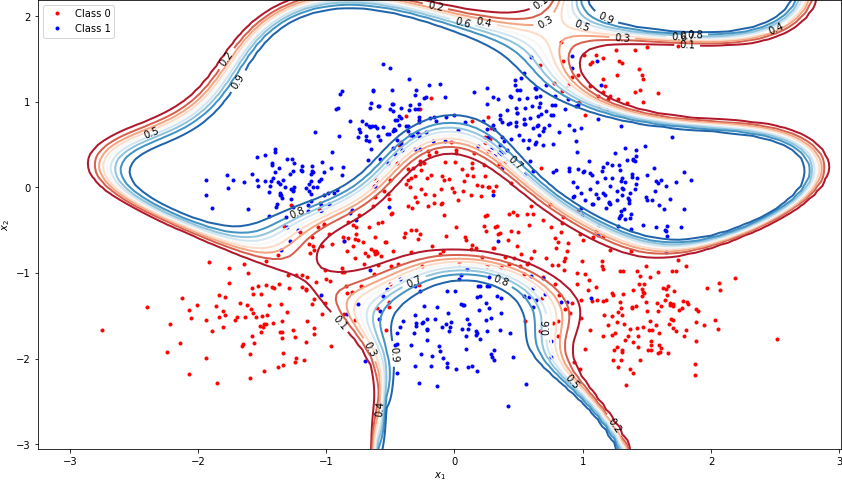
\includegraphics[width=\textwidth]{plots/bayesian_logistic_classification/predictive_distribution_ML_width_1}
            \caption{Maximum Likelihood estimate}
            \label{fig:predictive-distribution-ml-width-1}
        \end{subfigure}
        \begin{subfigure}{0.33\textwidth}
            \centering
            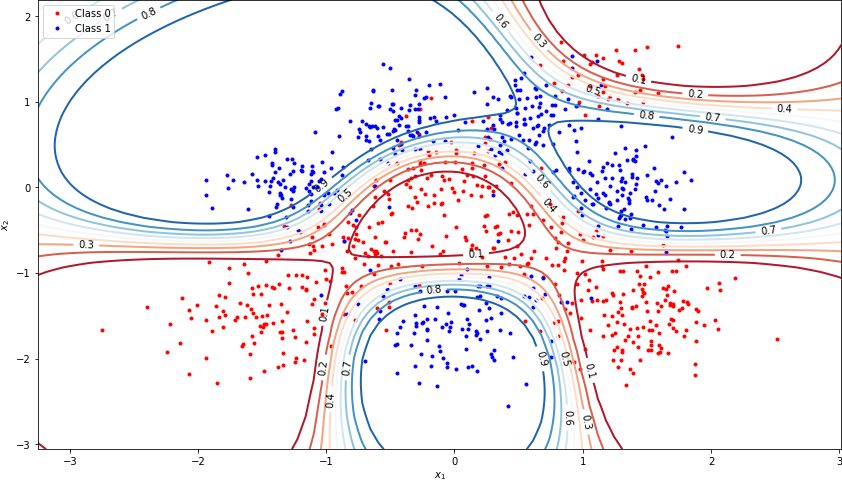
\includegraphics[width=\textwidth]{plots/bayesian_logistic_classification/predictive_distribution_MAP_width_1_prior_variance_1}
            \caption{MAP estimate ($\sigma_0^2=1$)}
            \label{fig:predictive-distribution-map-width-1}
        \end{subfigure}
        \begin{subfigure}{0.33\textwidth}
            \centering
            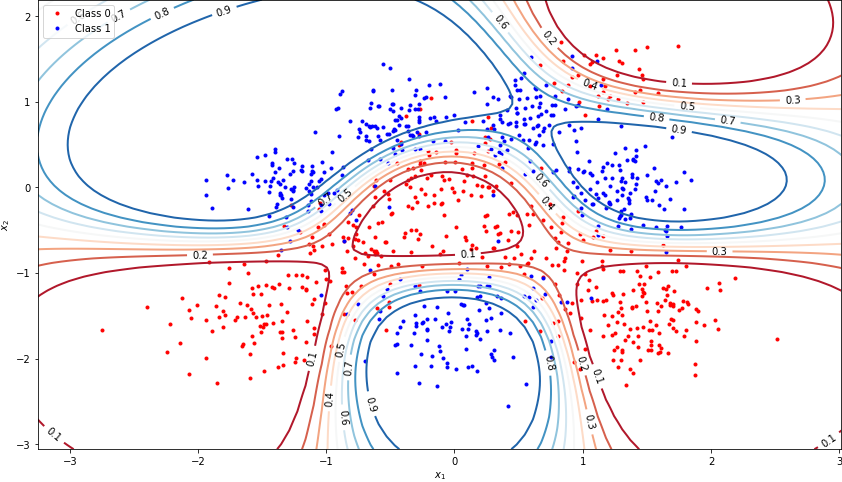
\includegraphics[width=\textwidth]{plots/bayesian_logistic_classification/predictive_distribution_laplace_width_1_prior_variance_1}
            \caption{Laplace approximation ($\sigma_0^2=1$)}
            \label{fig:predictive-distribution-laplace-width-1}
        \end{subfigure}
        \caption{Predictive distributions, RBF width = $1$}
        \label{fig:predictive-distributions-width-1}
    \end{figure}

    \subsubsection{Confusion matrices}
    To find the predicted class label for a point $\bm{x}_*$, a hard threshold is applied to the predicted class probabilities:
    \begin{align*}
        \hat{y} = \begin{cases}
                        0 & p(y_* = 1 | \bm{x}_*, \bm{y}, \bm{X}) \leq 0.5 \\
                        1 & p(y_* = 1 | \bm{x}_*, \bm{y}, \bm{X}) > 0.5
                    \end{cases}
    \end{align*}
    The threshold is applied to the predictive function evaluated on the test set.
    The performance of the classifier can be evaluated using the confusion matrix:
    \begin{align*}
        \begin{pmatrix}
                 P(\hat{y}=0 | y=0) & P(\hat{y}=1 | y=0) \\
                 P(\hat{y}=0 | y=1) & P(\hat{y}=1 | y=1) \\
        \end{pmatrix}
    \end{align*}
    The confusion matrices for the ML, MAP, and Laplace classifier are shown in \autoref{tab:confusion-matrices}.

    \begin{table}[h]
        \centering
        \begin{tabular}{c c}
            \textbf{Classifier} & \textbf{Confusion matrix} \\
            \hline
            ML estimate &
            $\begin{pmatrix}
                0.890 & 0.110 \\
                0.209 & 0.791 \\
            \end{pmatrix}$ \\
            MAP estimate &
            $\begin{pmatrix}
                0.908 & 0.092 \\
                0.132 & 0.868 \\
            \end{pmatrix}$ \\
            Laplace approximation &
            $\begin{pmatrix}
                0.908 & 0.092 \\
                0.132 & 0.868 \\
            \end{pmatrix}$ \\
        \end{tabular}
        \caption{Confusion matrices for different classifiers, with RBF width = 0.1 and $\sigma_0^2=1$}
        \label{tab:confusion-matrices}
    \end{table}

    The hard-thresholding operation renders the MAP and Laplace predictions identical, as the location of the decision boundary ($p(y_* = 1 | \bm{x}_*, \bm{y}, \bm{X}) = 0.5$) is the same in both cases.
    \autoref{tab:confusion-matrices} illustrates that the Bayesian classifier has improved performance compared to the likelihood-based classifier, with correct prediction percentage on the test set increased by by 1.8 and 7.7 percentage points for class 1 and class 2 respectively.
    This is due to the inclusion of the prior on the model weights, which acts to regularise the model by penalising large magnitude weights to reduce overfitting.

    \subsubsection{Log-likelihood}
    The log-likelihood is another metric for assessing the classifier performance, as a model that is fit well to the data should exhibit a more positive log-likelihood.
    It can be evaluated on the training and test sets which gives insight into whether the model has been overfitted to the training data.
    The log-likelihood for the Bayesian classifier (the likelihood is the same for the MAP and Laplace cases) is compared to the ML classifier in \autoref{tab:log-likelihood-performance}.
    The ML classifier has clearly been overfitted to the training data, as the log-likelihood is very close to zero for the training set and a large negative number for the test set.
    The Bayesian classifier exhibits slightly worse performance on the test set, which is to be expected, but the log-likelihood is of a similar magnitude for both training and test data.
    \begin{table}[h]
        \centering
        \begin{tabular}{c c c}
            & \multicolumn{2}{c}{\textbf{Mean log-likelihood}} \\
            &  \textbf{Training data} & \textbf{Test data} \\
            \hline
            ML estimate & $9.986 \times 10^{-6}$ & -1.785 \\
            MAP estimate & -0.2146 & -0.3108
        \end{tabular}
        \caption{Log-likelihood for the ML and MAP classifiers, with RBF width = 0.1 and $\sigma_0^2=1$}
        \label{tab:log-likelihood-performance}
    \end{table}

    \subsection{Optimising the hyperparameters}\label{sec:optimisation}
    The classifier we have implemented has two hyperparameters: \verb`rbf_width` and \verb`prior_variance`. The optimal setting for these parameters can be found by maximising the model evidence. We perform a grid search to find the maximum model evidence:
    \begin{minted}{python}
    def grid_search(rbf_widths, prior_variances):
        grid = np.empty((len(rbf_widths), len(prior_variances)))
        for i, rbf_width in enumerate(rbf_widths):
            for j, prior_variance in enumerate(prior_variances):
                expanded_X_train = expand_inputs(rbf_width, X_train)
                w_map = find_w_map(expanded_X_train, y_train, prior_variance)
                grid[i][j] = log_evidence(w_map, expanded_X_train, y_train,
                                          rbf_width, prior_variance)
    \end{minted}
    Initially, a coarse grid is used to find the appropriate range to optimise over (\autoref{fig:coarse-grid-evidence}).
    The most promising range is identified to be $0.1 < \sigma_0^2 < 10$, $0.01 < \text{RBF width} < 10$.
    It is also observed that for large prior variances ($\sigma_0^2 \geq 10$) the evidence cannot be computed - shown as white on the heatmap - as the covariance matrix $\bm{S}_N$ is no longer full rank.
    \begin{figure}[h]
        \begin{subfigure}{0.45\textwidth}
            \centering
            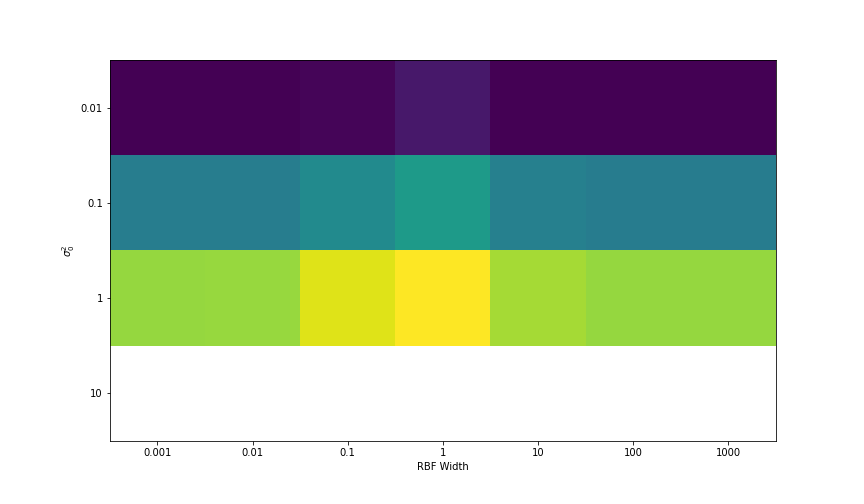
\includegraphics[width=\textwidth]{plots/bayesian_logistic_classification/coarse_grid_evidence.png}
            \caption{Coarse heatmap}
            \label{fig:coarse-grid-evidence}
        \end{subfigure}
        \hfill
        \begin{subfigure}{0.5\textwidth}
            \centering
            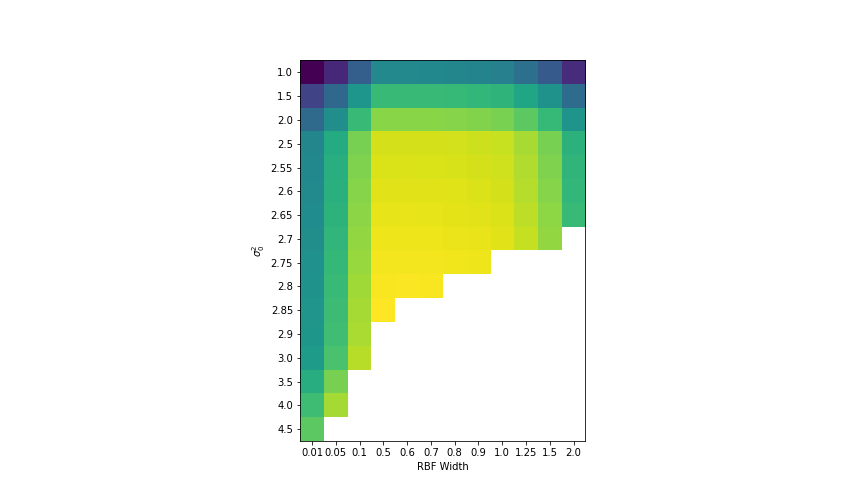
\includegraphics[width=\textwidth]{plots/bayesian_logistic_classification/fine_grid_evidence.png}
            \caption{Fine heatmap}
            \label{fig:fine-grid-evidence}
        \end{subfigure}
        \caption{Heatmaps of the model evidence for different settings of the hyperparameters}
    \end{figure}
    A finer grid search is performed within the optimal region (\autoref{fig:fine-grid-evidence}).
    The gradient of the evidence around the maximum is quite shallow, so there are a number of settings of the hyperparameters that could give good results.

    We choose a pair of values that are close to the center of the peak: $\sigma_0^2 = 2.8$, RBF width $= 0.7$.

    \subsubsection{Predictive distribution}
    The MAP estimate and Laplace approximation of the predictive distribution for this setting are shown in \autoref{fig:predictive-distribution-optimised}.
    The Laplace approximation is visibly a better fit to the data than the approximate predictive distributions generated before optimisation (compare \autoref{fig:predictive-distribution-optimised-laplace} to \autoref{fig:predictive-distribution-laplace-width-0.1} and \autoref{fig:predictive-distribution-laplace-width-1}).
    The advantages of the Laplace approximation over the MAP estimate, namely shallower boundaries and a tighter fit to data, have increased after optimisation (compare \autoref{fig:predictive-distribution-optimised-map} to \autoref{fig:predictive-distribution-optimised-laplace}).
     \begin{figure}[h]
         \begin{subfigure}{0.45\textwidth}
            \centering
            \includegraphics[width=\textwidth]{plots/bayesian_logistic_classification/predictive_distribution_map_width_0.7_prior_variance_2.8}
            \caption{MAP estimate}
            \label{fig:predictive-distribution-optimised-map}
         \end{subfigure}
         \hfill
    \begin{subfigure}{0.45\textwidth}
            \centering
            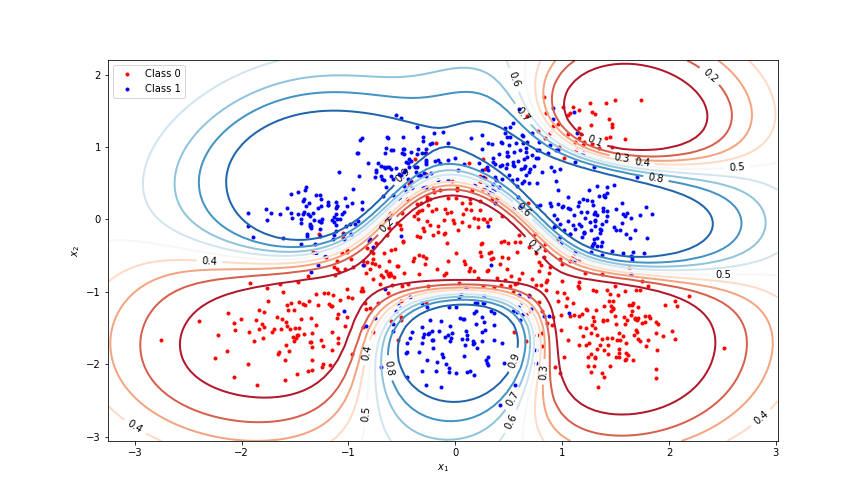
\includegraphics[width=\textwidth]{plots/bayesian_logistic_classification/predictive_distribution_laplace_width_0.7_prior_variance_2.8}
            \caption{Laplace approximation}
            \label{fig:predictive-distribution-optimised-laplace}
         \end{subfigure}
         \caption{Predictive distributions for $\sigma_0^2 = 2.8$, RBF width $= 0.7$}
         \label{fig:predictive-distribution-optimised}
    \end{figure}

    \subsubsection{Confusion matrix}
    The confusion matrix after hyperparameter optimisation is compared with the initial confusion matrix in \autoref{tab:confusion-matrices-optimised}.
    Optimising the hyperparameters has improved the classifier's ability to detect class 2 by 5.5 percentage points, at the cost of reducing its ability to detect class 1 by 1 percentage point.
    This is not as good an improvement as might be expected from the optimisation of the hyperparameters, so it would be beneficial to perform a more in-depth search for optimal settings.
    Due to computing time constraints, this will not be done in this report.
    \begin{table}[h!]
        \centering
        \begin{tabular}{c c c c}
            & $\sigma_0^2$ & \textbf{RBF width} & \textbf{Confusion matrix} \\
            \hline
            Before optimisation & 1 & 0.1 &
            $\begin{pmatrix}
                0.908 & 0.092 \\
                0.132 & 0.868 \\
            \end{pmatrix}$ \\
            After optimisation & 2.8 & 0.7 &
            $\begin{pmatrix}
                0.890 & 0.110 \\
                0.077 & 0.923 \\
            \end{pmatrix}$ \\
        \end{tabular}
        \caption{Confusion matrices for Laplace classifier before and after hyperparameter optimisation}
        \label{tab:confusion-matrices-optimised}
    \end{table}

    \subsubsection{Log-likelihood}
    The log-likelihood after hyperparameter optimisation is compared with the initial log-likelihood in \autoref{tab:log-likelihood-performance-optimised}.
    It can be seen that the log-likelihood has been improved (made more positive) by hyperparameter tuning and overfitting has still been avoided.
    \begin{table}[h!]
        \centering
        \begin{tabular}{c c c c c}
            & & & \multicolumn{2}{c}{\textbf{Mean log-likelihood}} \\
            &  $\bm{\sigma_0^2}$ & \textbf{RBF width} & \textbf{Training data} & \textbf{Test data} \\
            \hline
            Before optimisation & 1 & 0.1 & -0.2146 & -0.3108 \\
            After optimisation & 2.8 & 0.7 & -0.1742 & -0.2490
        \end{tabular}
        \caption{Log-likelihood for Bayesian classifier before and after hyperparameter optimisation}
        \label{tab:log-likelihood-performance-optimised}
    \end{table}

    \section{Conclusion}
    Extending a logistic classifier to a fully Bayesian approach has significant advantages over a maximum-likelihood classifier, as the prior distribution of the model weights can be used to reduce overfitting.
    The Laplace approximation is used to find an approximate posterior distribution of the weights and approximate the model evidence.
    The predictive distribution generated by the Laplace approximation outperforms the ML and MAP estimates in classifying new data points.
    The model evidence can be used to assess a model's performance, and is used to optimise the settings of the hyperparameters in the Bayesian logistic classifier with marginal gains in performance.
    One drawback of this approach is the high compute cost, as calculating the approximate model evidence is an intensive calculation.
    Further optimisation of the hyperparameters would likely show some improvement, but probably not at a significant level due to the shallow gradient of the evidence.
\end{document}
